\documentclass[conference]{IEEEtran}

% --- IDIOMA ---
\usepackage[spanish, es-tabla]{babel}

% --- FUENTES (XeLaTeX) ---
\usepackage{fontspec}
\setmainfont{Liberation Serif}
\setmonofont{JetBrainsMono Nerd Font}

% --- CITAS IEEE ---
\usepackage[backend=biber,style=ieee,sorting=none]{biblatex}
\addbibresource{referencias.bib}

% --- UTILIDADES ---
\usepackage{graphicx}
\usepackage{float}
\usepackage{amsmath}
\usepackage{booktabs}
\usepackage[colorlinks=true,linkcolor=black,citecolor=black,urlcolor=blue]{hyperref}

% --- CÓDIGO ---
\usepackage{xcolor}
\definecolor{bg}{RGB}{40,44,52}

\usepackage{minted}

\setminted{
  style=monokai,
  bgcolor=bg,
  breaklines,
  breakanywhere=true,
  tabsize=2,
  fontsize=\footnotesize
}

\usepackage{csquotes}

\begin{document}



% --- INICIO DE LA PORTADA ---
\begin{titlepage}
    \centering
    \vspace*{0.5cm}
    
    % --- Escudo de la UV ---
    % Asegúrese de tener el archivo escudo_uv.png (o .jpg) en su carpeta del proyecto
    
\includegraphics[width=0.3\textwidth]{UV.png} \\ 
    \vspace{0.8cm}
    
    {\huge \textbf{Universidad Veracruzana}} \\
    \vspace{0.4cm}
    {\Large Facultad de Instrumentación Electrónica} \\ % Corregido: Instrumentación
    \vspace{0.2cm}
    {\large Ingeniería Biomédica} \\
    
    \vfill
    
    % Título de la Experiencia Educativa y Actividad
    {\Large \textbf{EE: Interfaces Hombre-Máquina}} \\
    \vspace{0.8cm}
    {\Large \textbf{ACTIVIDAD 06. ACTUADORES EN EL PROCESO DE SALIDA DE INFORMACION DE UNA INTERFAZ HOMBRE-MAQUINA}} \\
    
    \vspace{1.5cm}
 
    % Información de los Integrantes
    \begin{flushright} % Alineado a la derecha para un toque más profesional
        \textbf{Profesor:} \\
        Varela Lara Luis Julian \\
        \vspace{0.5cm}
        \textbf{Integrantes del equipo ``\textit{ES3.14}}'': \\
        Alfonso Gamboa Rubén \\
        Flores Montero Edsel Yetlanezi \\
    \end{flushright}
    
    \vfill
    
    {\large \textbf{Fecha:} 20 de mayo de 2026} \\
    \vspace{1cm}
    {\small Xalapa, Enríquez, Ver.} % O la sede correspondiente
\end{titlepage}
% --- FIN DE LA PORTADA ---



% --- EL CUERPO DEL TEXTO (Automáticamente en dos columnas) ---

\section{Introducción al tema.}

 \subsection{Marco teórico}


\section{Desarrollo de la actividad.}
  \subsection{Librerías.}
  
  \subsection{Desarrollo del código.}

  \subsubsection{setup()}

  \subsubsection{loop()}


  \subsection{Código completo}
    A continuación se deja el código completo usado durante el desarrollo de esta actividad:
    \inputminted{cpp}{Act06.ino}
  \newpage
  
  \subsection{Armado de Circuito}
    \begin{figure}[h]
      \centering
      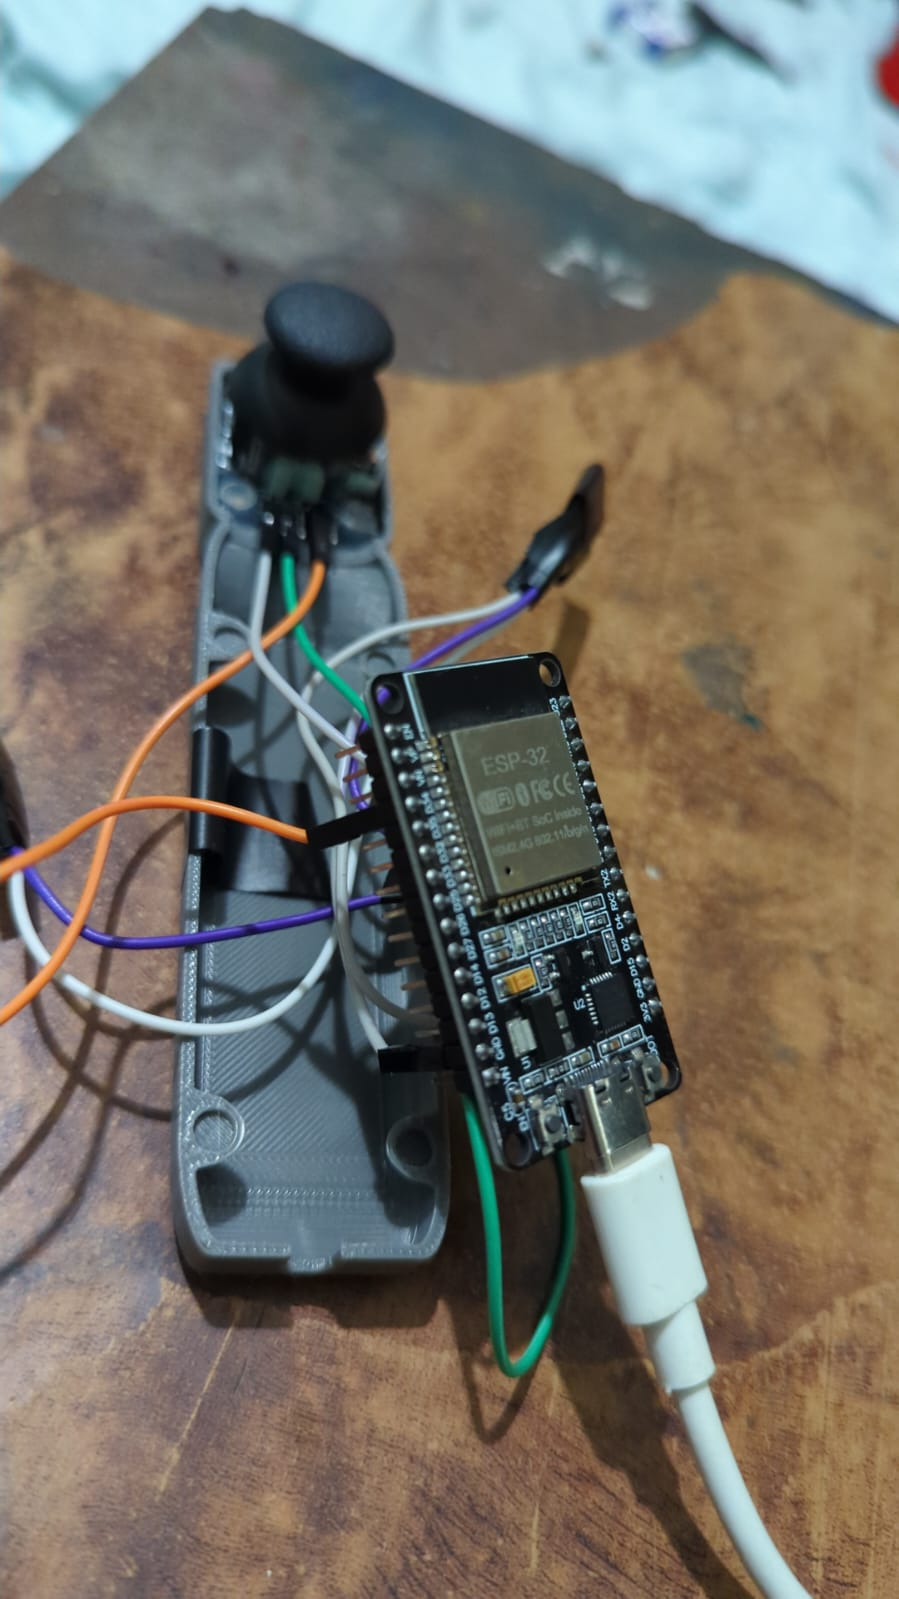
\includegraphics[width=\linewidth]{circuito.jpeg} % \linewidth se ajusta a la columna
      \caption{Vista general del circuito armado}
      \label{fig:circuito}
    \end{figure}

  \subsection{Conexiones y pines}
  \begin{itemize}
    \item 
  \end{itemize}

  



\section{Conclusiones}


\newpage{}
\section{firma de revisión}
\begin{figure}[h]
    \centering
    \includegraphics[width=\linewidth]{Firma.jpeg} % \linewidth se ajusta a la columna
    \caption{Firma de revisión}
    \label{fig:Firma}
\end{figure}




% --- REFERENCIAS ---
\printbibliography



\end{document}
